\documentclass[12pt, a4paper, oneside]{ctexart}
\usepackage[margin=1in]{geometry}
\usepackage{amsmath,caption, amsthm, amssymb, bm, color, framed, graphicx, hyperref, mathrsfs, listings, lmodern}
\usepackage{palatino}
\usepackage{fontspec}
\setmonofont{Consolas}

\lstset{
    basicstyle=\ttfamily\small,
    numbers=left,
    numberstyle=\ttfamily\footnotesize,
    stepnumber=1,
    numbersep=10pt,
    frame=none,
    xleftmargin=41pt,
    breaklines=true,
    tabsize=4,
    commentstyle=\color{gray},
    keywordstyle=\color{blue},
}
\title{\textbf{寻找样本DNA序列中的重复片段\\ 实验文档}}
\author{俞舜云\quad24300240045}
\date{2025年3月27日}
\linespread{1.5}
\definecolor{shadecolor}{RGB}{241, 241, 255}
\newcounter{problemname}
\newenvironment{problem}[1][]{%
\def\temp{#1}%
\ifx\temp\empty
	\stepcounter{problemname}%
	\def\problemLabel{\arabic{problemname}}%
\else
	\def\problemLabel{#1}%
\fi
\begin{shaded}\par\noindent{\textbf{题目\problemLabel \text{ }}}\kaishu
}{%
\end{shaded}\par
}
\newenvironment{solution}{\par\noindent\textbf{解答. }}{\par}
\newenvironment{proove}{\par\noindent\textbf{证明. }}{\par\noindent\textbf{得证. }\par}
\newenvironment{note}{\par\noindent\textbf{题目\arabic{problemname}的注记. }}{\par}
\newenvironment{textt}{\par\noindent}{\par}
\renewcommand{\labelenumi}{(\arabic{enumi})}

\begin{document}

	\maketitle

    \section{算法伪代码}
    本实验以动态规划算法为核心,通过以下几个核心步骤完成序列比对与重复区域识别:

    \subsection{预处理阶段}
    \begin{lstlisting}[language=Algol, basicstyle=\small\ttfamily]
Procedure PREP_ANALYZE(reference, query, kmer_size)
    // 初始化长度参数
    refeLength ← |reference| - kmer_size + 1
    querLength ← |query| - kmer_size + 1
    
    // 计算哈希值
    refeHash ← ROLLING_HASH(reference)
    querHash ← ROLLING_HASH(query)
    refeRevHash ← ROLLING_HASH(REVERSE_COMPLEMENT(reference))
    
    // 初始化动态规划表
    for i ← 0 to querLength - 1 do
        for j ← 0 to refeLength - 1 do
            Align[i][j] ← (MIN_INF, -1, 0)
        end for
    end for
    
    Align[0][0] ← (0, -1, 1)
    
    // 初始化查询序列对齐数组
    for i ← 0 to querLength - 1 do
        querAlign[i] ← (MIN_INF, -1, -1)
    end for
    
    querAlign[0] ← (0, 0, -1)
    
    // 初始化路径记录结构
    for i ← 0 to querLength - 1 do
        pointRoute[i] ← (0, -1, 0)
    end for
end Procedure
        \end{lstlisting}
        
        \begin{lstlisting}[language=Algol, basicstyle=\small\ttfamily]
Procedure ANALYZE_ROUTE(reference, query)
    // 主循环,遍历每个查询序列位置
    for i ← 1 to querLength - 1 do
        for j ← 0 to refeLength - 1 do
            // 考虑正向匹配
            if IS_EQUAL(i, j) then
                // 新开序列得分
                Align[i][j] ← (querAlign[i-1].maxScore + maintainScore + newScore, 
                                querAlign[i-1].maxScoreIndex, 1)
                
                // 继续延续得分
                if j - 1 ≥ 0 and IS_EQUAL(i-1, j-1) then
                    if Align[i][j].maxScore < Align[i-1][j-1].maxScore + 
                                            maintainScore + 
                                            Align[i-1][j-1].continuousCount * continuousScore then
                        Align[i][j] ← (Align[i-1][j-1].maxScore + 
                                        maintainScore + 
                                        Align[i-1][j-1].continuousCount * continuousScore,
                                        j-1, Align[i-1][j-1].continuousCount + 1)
                    end if
                end if
                
                // 更新当前查询位置的最佳匹配
                if querAlign[i].maxScore < Align[i][j].maxScore then
                    querAlign[i] ← (Align[i][j].maxScore, j, Align[i][j].prevIndex)
                end if
            
            // 考虑反向互补匹配
            else if IS_MATCH(i, j) then
                // 类似正向匹配的处理,但参数和方向不同
                // 略...
            end if
        end for
    end for
end Procedure
        \end{lstlisting}
        
        \begin{lstlisting}[language=Algol, basicstyle=\small\ttfamily]
Procedure ANALYZE_SEQUENCE()
    // 回溯得到最优路径
    h ← querLength - 1
    l ← refeLength - 1
    while h ≥ 0 and l ≥ 0 do
        Route[h][l] ← Align[h][l].maxScore
        pointRoute[h] ← (Align[h][l].maxScore, l, Align[h][l].prevIndex)
        l ← Align[h][l].prevIndex
        h ← h - 1
    end while
    
    // 提取连续子串
    head ← 0
    while head < querLength do
        tail ← head + 1
        // 寻找连续序列的终点
        while tail < querLength and |Align[tail][pointRoute[tail].maxScoreIndex].continuousCount| ≠ 1 do
            tail ← tail + 1
        end while
        
        // 创建重复序列片段
        if IS_MATCH(head, pointRoute[head].maxScoreIndex) then
            segment ← CREATE_SEGMENT(query[head:tail-1], 
                                    pointRoute[head].maxScoreIndex,
                                    tail-head, 1, true, head, tail-1)
            segments.APPEND(segment)
        else
            // 处理非匹配情况
            // 略...
        end if
        
        head ← tail
    end while
end Procedure
        \end{lstlisting}
        
        \begin{lstlisting}[language=Algol, basicstyle=\small\ttfamily]
        Procedure LINEAR_SEARCH(A, v)
            for i ← 1 to |A| do
                if A[i] = v then
                    return i
                end if
            end for
            return NIL              
        end Procedure
        \end{lstlisting}

    \section{时空复杂度分析}
    
    假设参考序列长度为 $n$,查询序列长度为 $m$,分析各阶段的时空复杂度:
    
    \subsection{时间复杂度}
    
    \begin{enumerate}
        \item \textbf{预处理阶段}: 
        \begin{itemize}
            \item 滚动哈希计算:$O(n^2)$ 和 $O(m^2)$,用于计算所有子串的哈希值
            \item 初始化动态规划表:$O(nm)$,需要初始化 $m \times n$ 大小的表格
        \end{itemize}
        
        \item \textbf{序列比对阶段}: 
        \begin{itemize}
            \item 主循环:$O(nm)$,需要遍历查询序列的每个位置和参考序列的每个位置
            \item 每个位置的计算:$O(1)$,包括正向和反向匹配计算
        \end{itemize}
        
        \item \textbf{序列分析与提取阶段}: 
        \begin{itemize}
            \item 回溯路径:$O(m)$,最多需要回溯查询序列的长度
            \item 提取连续子串:$O(m)$,最多遍历整个查询序列
        \end{itemize}
    \end{enumerate}
    
    综合分析,算法的总时间复杂度为 $O(n^2 + m^2 + nm)$,当查询序列和参考序列长度相近时,时间复杂度约为 $O(n^2)$。
    
    \subsection{空间复杂度}
    
    \begin{enumerate}
        \item \textbf{哈希值存储}: 
        \begin{itemize}
            \item 参考序列哈希:$O(n^2)$
            \item 查询序列哈希:$O(m^2)$
        \end{itemize}
        
        \item \textbf{动态规划表}: 
        \begin{itemize}
            \item Align矩阵: $O(nm)$
            \item querAlign和pointRoute数组: $O(m)$
            \item Route矩阵: $O(nm)$
        \end{itemize}
        
        \item \textbf{结果存储}: 
        \begin{itemize}
            \item segments数组: $O(k)$,其中 $k$ 是识别出的序列段数量
        \end{itemize}
    \end{enumerate}
    
    综合分析,算法的总空间复杂度为 $O(n^2 + m^2 + nm)$,主要受哈希表和动态规划表的大小影响。

    \section{运行结果}

    对于样例 reference、query , 得到运行结果如下
    \begin{figure}[htbp]
        \centering
        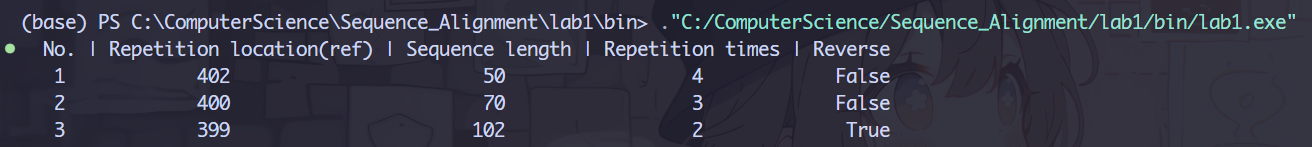
\includegraphics[width=0.8\textwidth]{运行结果.png}
        \caption{终端输出}
    \end{figure}

    \begin{center}
        \begin{lstlisting}[language=C, numbers=none, xleftmargin=40pt, frame=none, basicstyle=\scriptsize\ttfamily]
No. | Repetition location(ref) | Sequence length | Repetition times | Reverse
1            402                       50                 4            False
2            400                       70                 3            False
3            399                      102                 2             True
        \end{lstlisting}
        \captionof{figure}{终端输出text}
        \end{center}

    \begin{figure}[htbp]
        \centering
        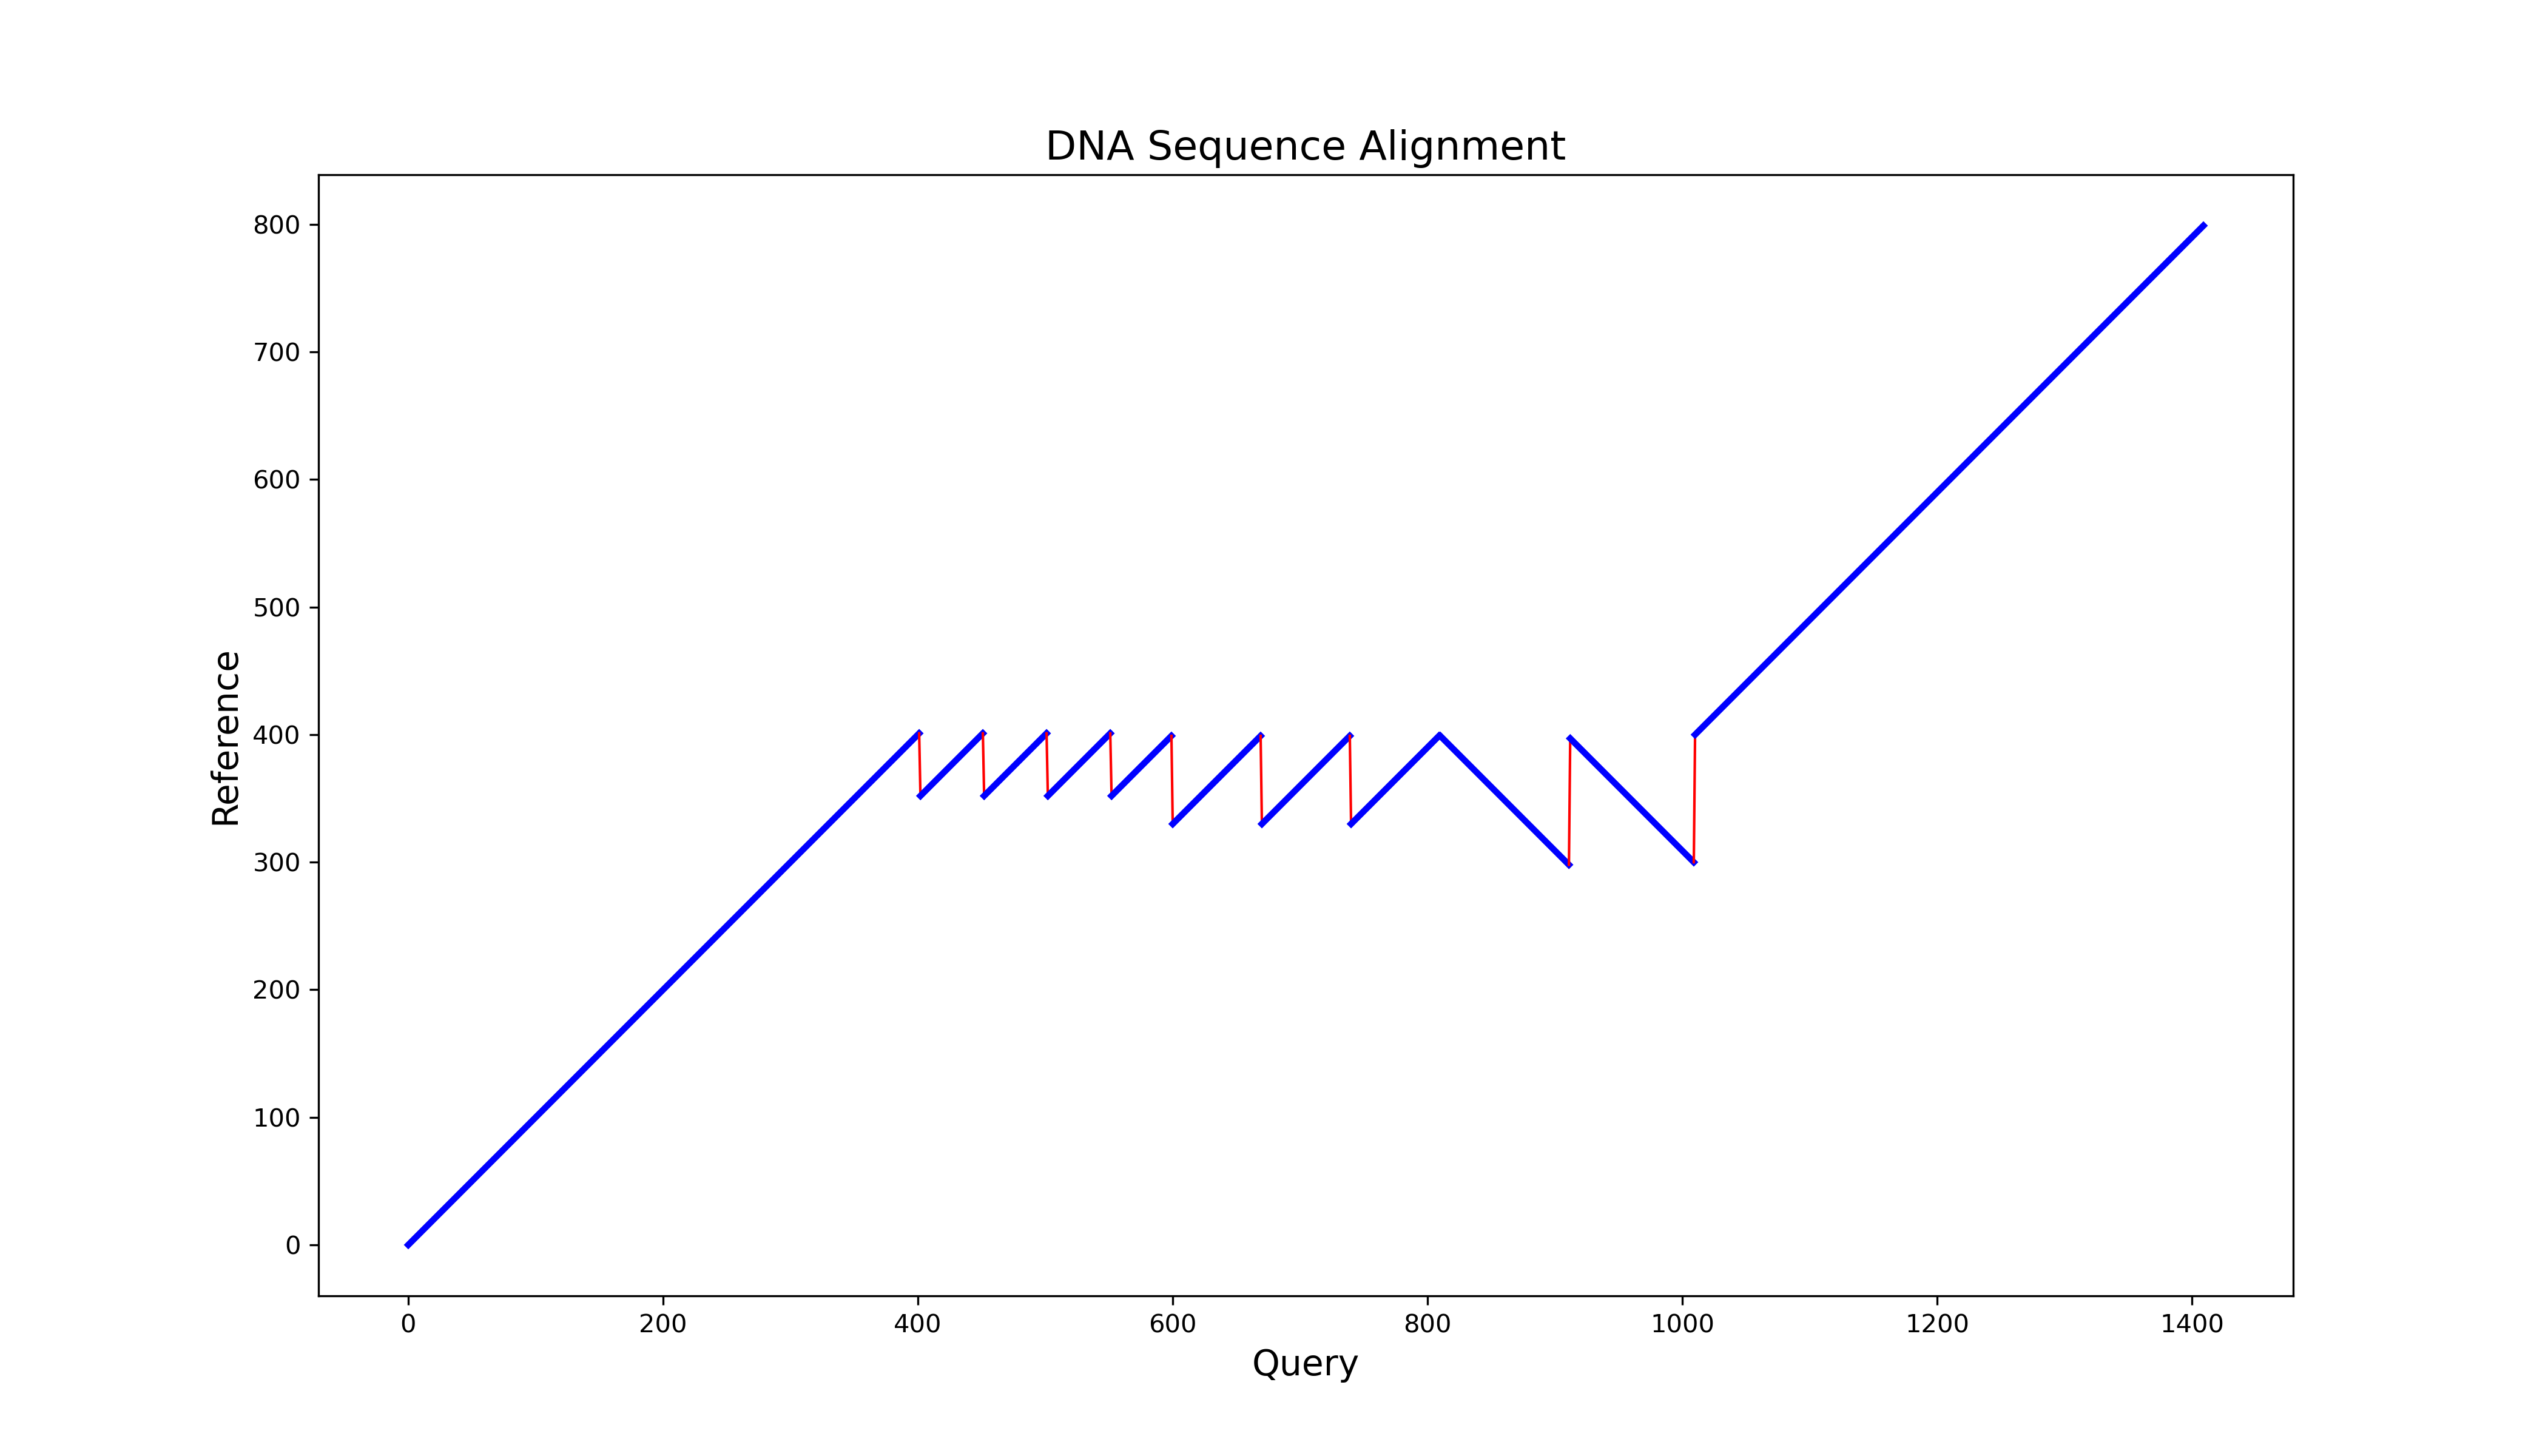
\includegraphics[width=0.8\textwidth]{演示图像.png}
        \caption{模拟比对演示}
    \end{figure}


		

\end{document}